\hoofdstuk{Background}
\paragraaf{Lunatech Research B.V}
Lunatech provides application development services, completely based on open-source web and Java technologies and open standards. They are early adopters of new technology, and use cutting-edge frameworks and tools to give themselves the advantage in software development. To stay up-to-date, their developers have the opportunity to research, try new technologies and contribute to open-source projects. The company is dominated by software developers. Everyone (except the director) writes code, on top of which some staff have a secondary management role, and the staff who will deliver a project interact with the customer directly.

\paragraaf{Rotterdam University of Applied Sciences (Hogeschool Rotterdam)}
Rotterdam University is one of the major Universities of Applied Sciences in the Netherlands. Currently almost 30,000 students are working on their professional future at our university.
The university is divided into eleven schools, offering more than 80 graduate and undergrad- uate programmes in seven fields: art, technology, media and information technology, health, behaviour and society, engineering, education, and of course, business.\cite{HogeschoolRotterdam2012}

\paragraaf{Stager}
In 2011, live music venue WORM - Instituut voor Avantgardistische Recreatie hired Lunatech to build Stager, a modern web-based resource planning and ticketing application to help manage live music events. Lunatech took the opportunity to use the relatively new Play framework to build a web application with an HTML5 and Java architecture. Stager has broad requirements ranging from high performance and security for the public ticket sales component, high usability for the internal resource planning component that will be used for hours a day by employees and being open to enhancements in the future for new customers.

\subparagraaf{WORM}

\hoofdstuk{Mobile platforms}

\paragraaf{Introduction}
% per platform: van wie is het, wat is de geschiedenis, waar wordt het gebruikt, welke achterliggende techniek drijft het?
The following chapter presents a concise overview of current mobile operating systems for mobile platforms, specifically smartphones and tablets.

A smartphone can be defined as a smart phone is a next-generation, multifunctional cell phone that provides voice communication and text-messaging capabilities and facilitates data processing as well as enhanced wireless connectivity.\cite{Ni2006}

\subparagraaf{Apple iOS}
iOS is a proprietary mobile operating system, developed by Apple Inc. It was originally released in 2007 for the iPhone and iPod Touch

\subparagraaf{Google Android}
Android is a opensource mobile operating system, developed by the Open Handset Alliance, led by Google and other companies.\cite{Inc.2012}

\subparagraaf{BlackBerry OS}
BlackBerry OS is a proprietary mobile operating system, developed by RIM\emph{(Research In Motion)} for its line of BlackBerry mobile devices.

\subparagraaf{Windows Phone 7}
Windows Phone 7 is a mobile operating system, developed Microsoft as a succesor to its Windows Mobile platform.

\subparagraaf{Java ME}

\subparagraaf{Symbian}

\paragraaf{Marketshares}

\begin{centering}
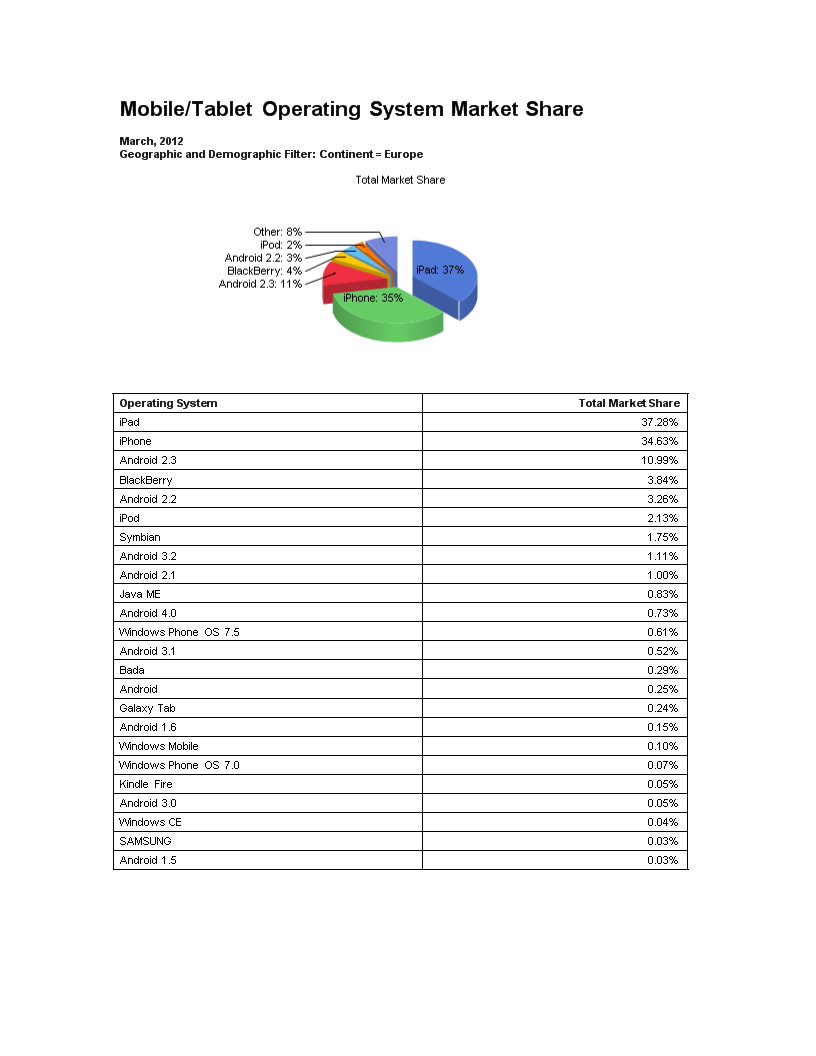
\includegraphics[scale=0.5]{images/netmarketshare_march2012.png}\\
\end{centering}

\begin{tabel}{|>\R p{\Procent{25}} | >\R p{\Procent{25}} |}{vbx}{Marketshare in the european continent as of march 2012\cite{Netmarketshare2012}}
\hline
\bf{Operating System} & \bf{Total \% Market Share}\\
\hline \hline
iOS & 74.04\\
Android & 18.36\\
BlackBerry & 3.84\\
Symbian & 1.75\\
Java ME & 0.83\\
Windows Phone & 0.68\\
Bada & 0.29\\
Windows Mobile & 0.14\\
Kindle & 0.05\\
Samsung & 0.03\\
LG & 0.01\\
ZTE & 0.00\\
Palm & 0.00\\
\hline
\end{tabel}

\hoofdstuk{Defining native}
\paragraaf{Intoduction}
The following chapter will define the \emph{native look-and-feel}.

\paragraaf{Native applications}
A native application is by definition an application inherent to the platform it was build for using techniques proprietary to the platform. For example, an iOS application is native when written in Objective-C. 


\subparagraaf{The native look}
%provided UI components \  homogeneous look to device OS \ 
When written in the native framework for a platform an mobile application receives acces to the available public libraries of the platform. These libraries include the UIKit\emph{(on iOS)} which provides the developer with a pre fabricated set of user interface components. These can be seen as the buildingblocks for an graphical userinterface on that platform. When used, the general style of the mobile application gains homogeneity to the overal user interface design of the platforms operating system. 

\subparagraaf{The native feel}
bounces \ solidity(not the whole app runs in a scrollview) \ view load speed \ view navigation animations \ 


\paragraaf{Comparison to web apps}
\paragraaf{Comparison to hybrid apps}

\hoofdstuk{Exsisting solutions to Cross-platform Mobile Application Development}
\paragraaf{Intoduction}
\paragraaf{PhoneGap}
\paragraaf{Appcelerator Titanium}
\paragraaf{Rhodes}
\paragraaf{Worklight}
\paragraaf{MoSync}
\paragraaf{Comparison}

\hoofdstuk{Developing cross-platform native applications with Titanium}
\paragraaf{Inner workings}

\hoofdstuk{Stager app requirements}

\hoofdstuk{Development and design}
\paragraaf{Stager app}
\subparagraaf{Events}
\subparagraaf{Notifications}
\subparagraaf{Tickets}
\subparagraaf{Mobile payment}
\paragraaf{Titanium modules}
\paragraaf{Stager service modules}









